\documentclass[a4paper,12pt,english]{article}
\usepackage[nottoc,numbib]{tocbibind}
\usepackage[utf8]{inputenc}
\usepackage[english]{babel}
\usepackage{amsmath}
\usepackage{amssymb}
\usepackage{listings}
\usepackage{booktabs}
\usepackage{graphicx}
\usepackage{makeidx}
\usepackage{titlesec}
\usepackage{fancyhdr}
\usepackage{wrapfig}
\usepackage{fancyvrb}
\usepackage{pbox}
\usepackage{hyperref}
\usepackage{mathtools}
\usepackage{amsmath}
\usepackage{multicol}
\usepackage{tocloft}%
\usepackage[refpage]{nomencl}
\usepackage{etoolbox}
\usepackage{longtable}
\usepackage{hyperref}
\usepackage{color}
\usepackage{xcolor}
\apptocmd{\sloppy}{\hbadness 10000\relax}{}{}
\usepackage{nomencl}
\makenomenclature

\graphicspath{ {/} }
\pagestyle{fancy}
\lstset{language=C,
                basicstyle=\ttfamily,
                basicstyle=\small,
                keywordstyle=\color{blue}\ttfamily,
                stringstyle=\color{red}\ttfamily,
                commentstyle=\color{green}\ttfamily,
                morecomment=[l][\color{magenta}]{\#},
                breaklines=true
}

\setcounter{secnumdepth}{4}
\setcounter{tocdepth}{4}


%Setting link borders to none
\hypersetup{pdfborder = {0 0 0}}

\fancyhead[C]{}
\fancyhead[L]{}
\fancyhead[R]{\footnotesize{
Sebastian O. Jensen}}


\begin{document}
\pagenumbering{Alph}
\begin{titlepage}

\newcommand{\HRule}{\rule{\linewidth}{0.4mm}}
\center
\small{ \emph{Forfatter:}\\
14.06-79 Sebastian O. Jensen \textsc{GJX653}
} \\[2cm]

\textsc{\LARGE KEA}\\[0.5cm]
\textsc{\large}\\[1.5cm]
\textsc{\huge Nodejs}\\
\HRule \\[0.7cm]
{\bfseries Keywords: Node.js, MongoDB, Express, AngularJS, Docker,
RESTfull, Web service}\\[0.4cm]
\HRule
\\[1.5cm] \textsc{\Large \textsc{\today}}\\[0.5cm]

\end{titlepage}
\tableofcontents

\pagenumbering{arabic}

\clearpage
\subsection{Abbreviations}
\renewcommand{\nomname}{}
\renewcommand{\pagedeclaration}[1]{}
\pagestyle{empty}
\printnomenclature[3cm]
\clearpage
\section{Introduction}
\subsection{Abstract}
Forecasts say that in 2020 there will be 25 billion devices connected to the
Internet. In 2014 there was around 3.7 billion devices\cite{Gartner}.
This put a big demand on common technologies such as relational
databases, sessions bassed communication, etc. This project
is a part of a larger project that investigates how to deal with
these challenges. The project does this by designing a system that
meets these challenges. The system consists of multiple devices which connect
in a local network and send information to a backend system over the internet.
This is a realistic example of how to deal with the future of
IoT\nomenclature{IoT}{Internet of Things}. The application consist of the
following items
\begin{enumerate}
  \item Battery powered devices that communicate via the ZigBee protocol.
  \item ZigBee/Internet gateway.
  \item Backend developed using Node.js and the database MongoDB
  \item Frontend developed in AngularJS.
\end{enumerate}

This project is about the backend system (3) does only
loosely talk about the frontend (5) when this is needed to describe and show the
functionality of the backend. The devices (1) and gateway (1) will not be
described in this repport. 

\subsection{Overview of this report}
In section 1.3 is the background for the system described. Section 2 will give a
theoretical background on the technologies which will be used
to implement the backend. Section 3 will give a technical description on the
implementation. Section 4 contains the conclusion.

\subsection{Background}
Internet of Things is the term that describes networks of physical devices that
are connected to the Internet. This can be anything like sensors, wearables,
fridges, heating systems, light balls and what ever could be imagined to
connect to the Internet.
As mentioned there is a high growth in the number of these devices. This project
is about solving a common problem in leisure harbors. 
In leisure harbors there are a limited number of moorings. Therefor each boat
owner has his own mooring space. At each mooring space there are a sign which
can be set to red or green. When the owner leaves the harbor he should set the
sign to green indicating that the mooring is free to use for guests. If he is
away for less than a day he can set it to red indicating that the mooring is
not free to use. When the owner returns home after some days he calls the harbor
master who then flips the sign to red indicating that the mooring is no longer
free. A common problem is that the boat owners often don’t set the signs to
green when they leave the harbor. The reason is that it is easier to let it stay
red instead of calling the harbor master when returning home. This often results
in many unused moorings has red signs and makes it difficult for guests to find
free moorings. Another problem is the time the harbor master uses on flipping
the signs for people returning home to their berth.
To solve these problems a system of electronically controlled signs is
suggested. For more details about the suggested system refer to section 3.1


\section{Theoretical background}

\subsection{Database system}
\subsubsection{Relational database database}
Relational Database Management Systems (RDBMS)\nomenclature{RDBMS}{Relational
Database Management Systems}store date in tables. Access or modification to
data is done using a Structured Query Language (SQL)
\nomenclature{SQL}{Structured Query Language}It was developed in the 1970s and
has been the de facto standard for many years. 

\subsubsection{NoSQL database}
Doing the 2000s an alternative to the RDBMS start to become popular.
The the NoSQL Databases. NoSQL stands for ``not only SQL''.
\nomenclature{NoSQL}{not only SQL}There are different ways the NoSQL can store
data. But what they have in common is that they use an object orientated
approach. Some of the NoSQL databases are graph databases that are good at
handling graph data. This could be data in a social network about who is
connected to who. Other stores data in documents or wide-columns \cite{mongo}. 
A NoSQL database is often very easy to scale as the developer can just start up
another instance of the DB and the DB will then by it self distribute data among
the DB instances. With SQL DBs it is also possible to to divide data on more
servers. But due to the way data is stored this require more work to do. A NoSQL
DB is often many times faster than a SQL DB depending on the job it has to do.

\section{Design of the harbor system}
This section covers how the system is designed. The requirements of the
system is explained in the first section to give a detailed understanding of
what the system is intended to do. In section 3.3 the hardware components are
described and in 3.4 the implementation which cover the software are described.

\subsection{Requirements}
The functional requirements of the system is as follow.

\begin{itemize}
	\item The signs should automatically turn green when a boat leaves the mooring
	\item The signs should be operated from a remote platform. E.g. a web platform
	\item The signs should be wireless controlled and battery powered as it is
	      complicated and expensive to do cabling in the harbors.
	\item Each sign should be able to hold power for minimum of 7 years.
\end{itemize}

There are
many possibilities for adding functionality to the system such as setting a
predefined time when a sign should flip and let guest see which moorings is
free and for how long. But these functionalities should be implemented on the
server side and is therefore not considered important for this project as the
focus is on the wireless communication between the signs and interconnection
with the web platform/application server. The reason why these added
functionalities should be added on the server is for practical reasons. The
three main reasons are as follow

\begin{itemize}
  \item It is a lot easier to make changes to the code running on the server
  then it is to update the code on the devices.
  \item The devices has limited amount of processing power and memory
  \item The devices run on battery and therefore should do as little work as
  possible.
\end{itemize}  
  The sensor which should sense if there is a boat at the mooring is simulated
  by a switch and the red green indication is simulated with an led. Again this is do to
  keeping the focus around the communication between devices and application
  server and not on the hardware development.
\clearpage

\subsection{Architecture}
A detailed drawing of the architecture can be viewed in fig. \ref{uml} below.
Explanation of individual components will be given under each section below
\begin{figure}[h]
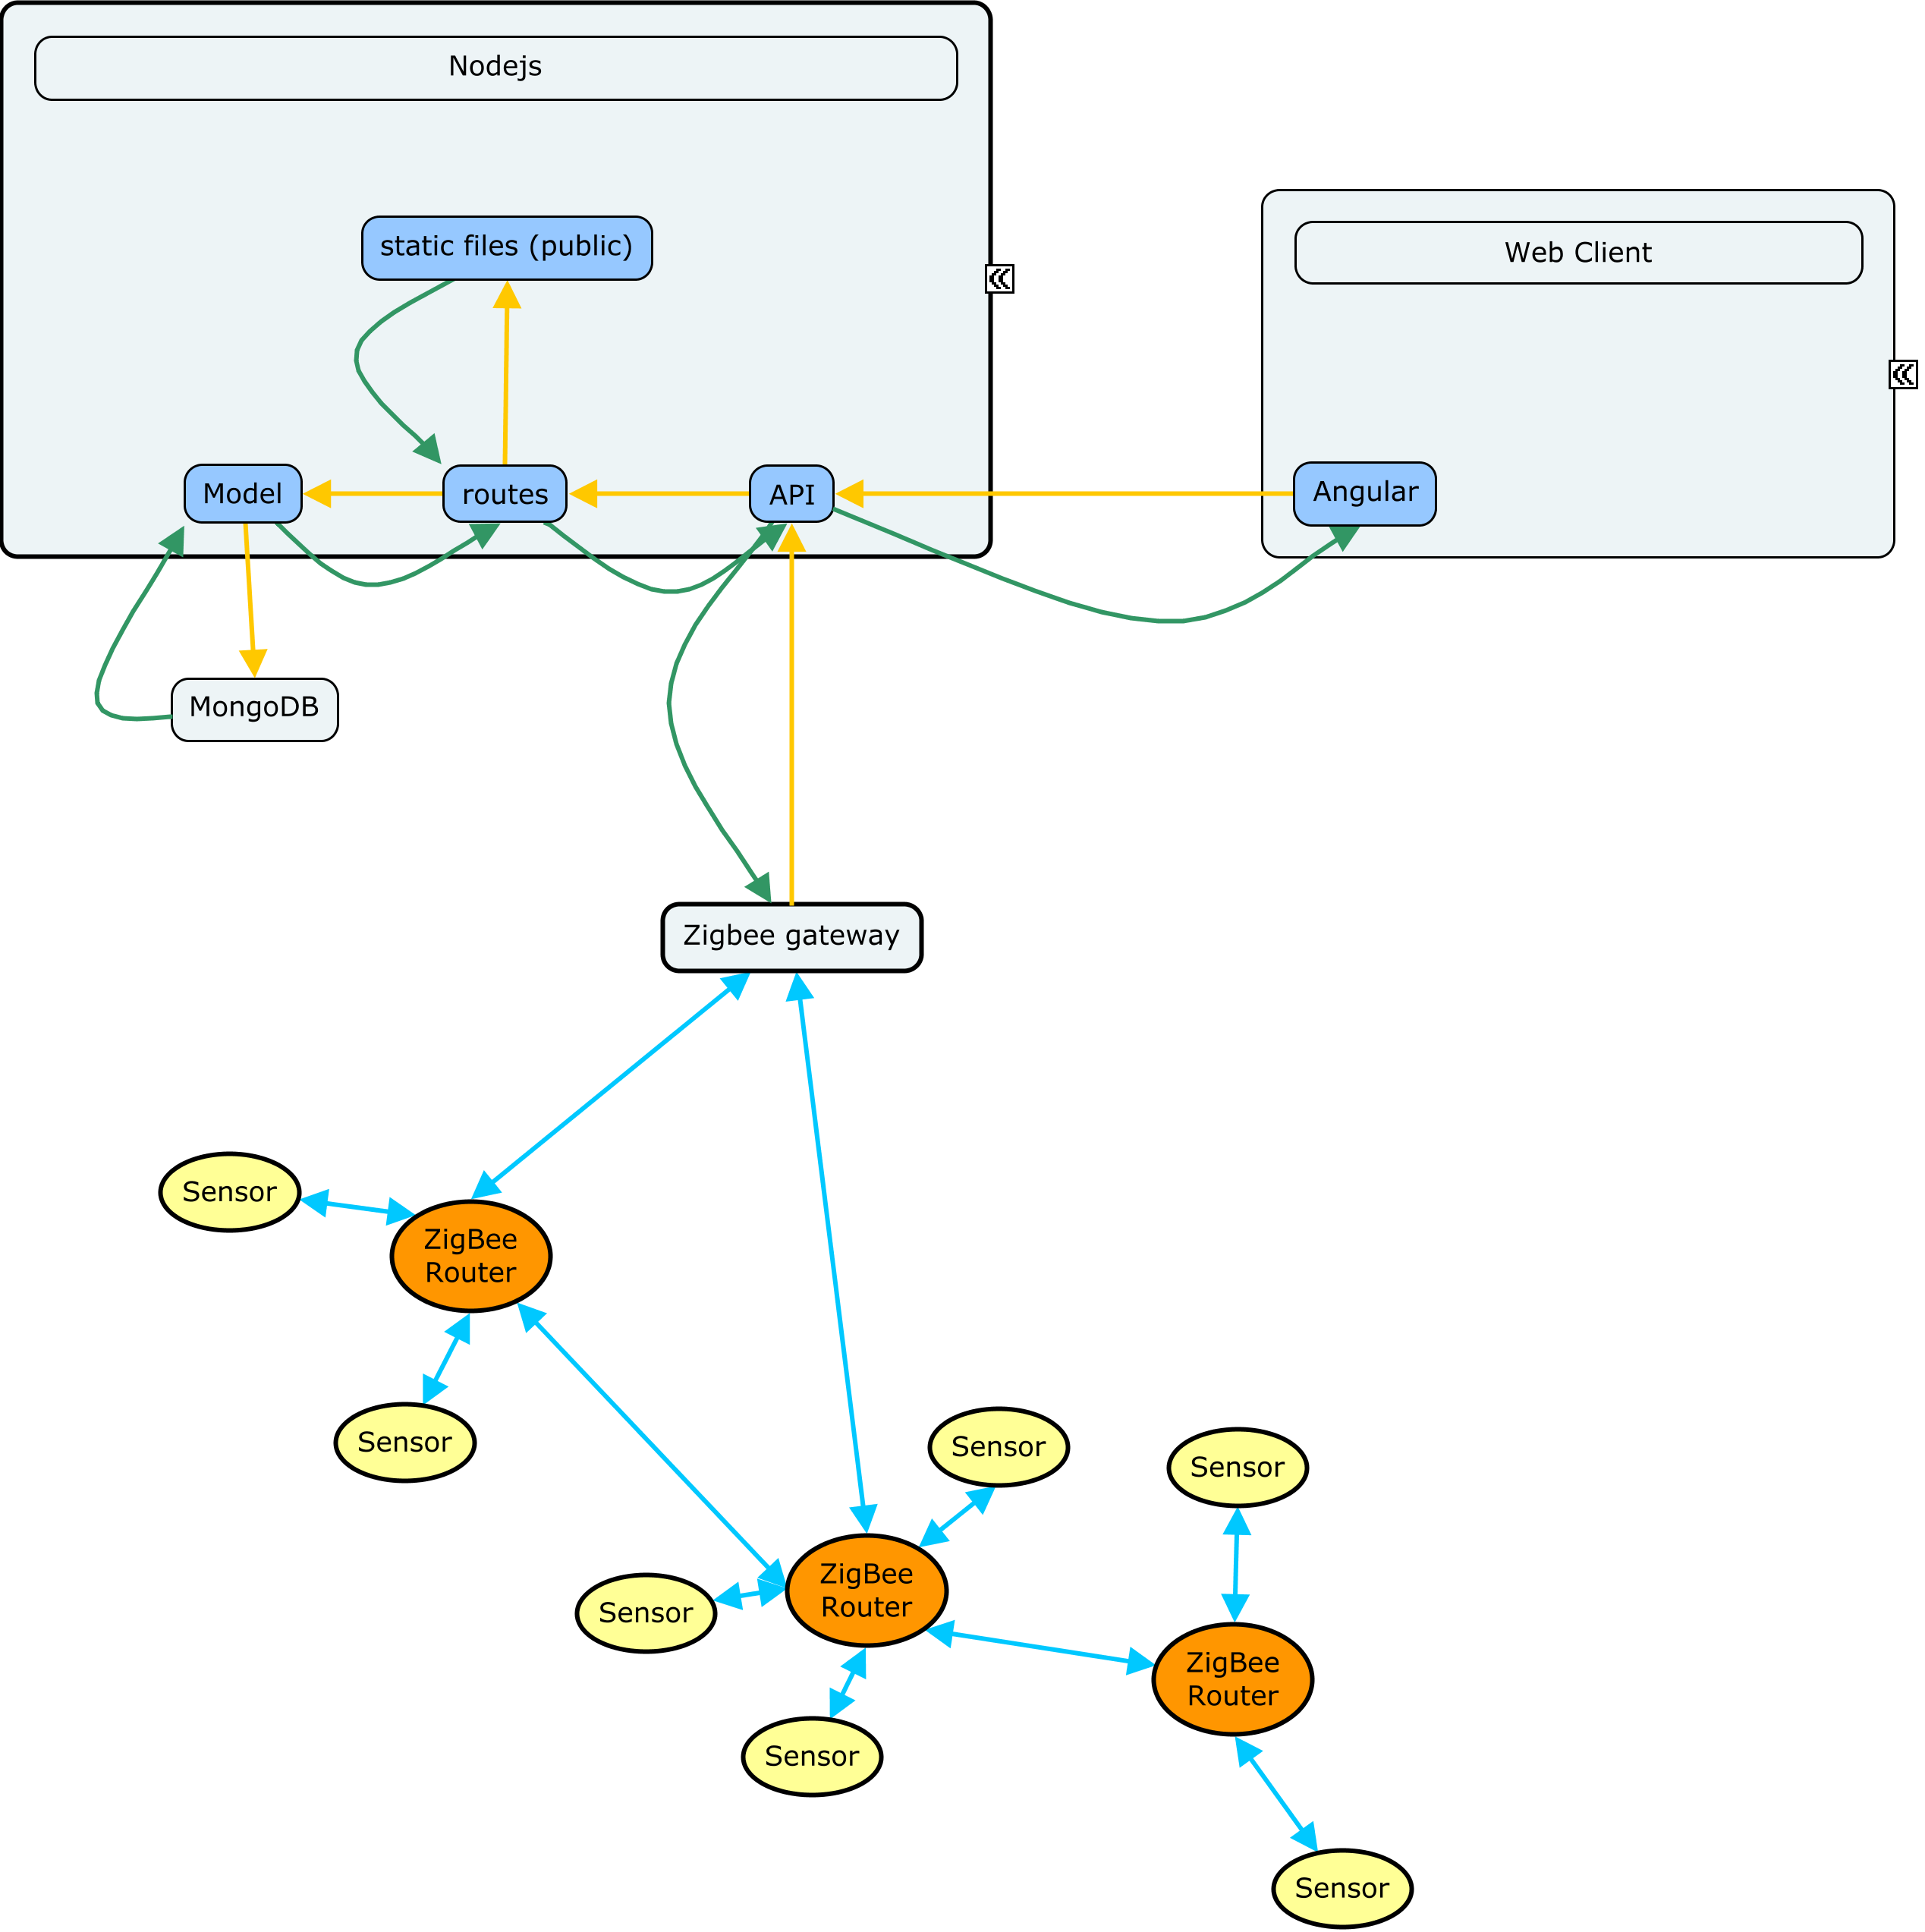
\includegraphics[scale=0.15	]{img/architecture.png}
\caption{Architecture}
\label{uml}
\end{figure}

\subsection{Hardware}
 
\subsubsection{Raspberry Pi}
A ZigBee network needs a gateway if the devices on the network need to
communicate with entities outside the ZigBee network. As we need
communication between the Signs on the ZigBee network and the application
server which is on the Internet we will need a gateway which translate
messages between those to networks. The Raspberry Pi can be used for this. A
Raspberry Pi is a small single board computer. You can run various Linux
distribution and even windows 10 on it. The latest version has a 900Mhz
quad-core ARM CPU and 1GB ram \cite{raspberry}. One thing that is useful
for this project is the GPIO pins. \nomenclature{GPIO}{General
purpose input output}The Raspberry Pi has 40 of them and they can be set up to
be used for different purpose. In this project will use it to interface with a
CC2530 over SPI \nomenclature{SPI}{Serial Peripheral Interface}. The Raspberry
Pi will also be connected to the Internet via a wifi dongle. A CC2530 module
has been bought from a Chinese manufacturer. This module is connected to the
Raspberry Pi. To connect the pins of the module and be able to make some
test with flipdots a test PCB has been produced. This PCB allows to easily
connect the CC2530 module to the Raspberry Pi via jumper cables. The PCB
connected to the Raspberry Pi can be seen in fig. \ref{pcb}. Some of the signals
runs over a breadboard with LED's for trouble shouting reasons.

\subsubsection{Application server}
The application server is setup on a virtual server at Amazon. Amazon has a
service called EC2 where you can rent servers in the cloud. For this project the
smallest instance is used. But the service let you easily scale up the server
is need be.

\subsection{Implementation}


\subsubsection{Application Server}
The Aplication server are not implemented jet but the purposed implementation is
explained in this section. Only a brief describtion of the pupposed tools are
provided as it is outside the scope of this project to go into details.

\paragraph{REST}
Communication between the Raspberry Pi and the application server should be
implemented using REST. REST stand for Representational State Transfer.
\nomenclature{REST}{Representational State Transfer}
One of the most important constraints in REST is it is stateless which means
that every request should contain all information to process the event. In this
session state is stored on the client which avoid the need for sessions. When
using sessions the server will need to hold information about all the devices
sessions while communicating. This makes it more difficoult to scale the system
as request can not so easely be load ballanced between multiple servers. Whith
rest load balancing is easy it does not matter to which server the request is
sent as the request holds all information to process the event.


\paragraph{MongoDB}
As descibed in the theoretical section a NoSQL database is often many times
faster than a relational database. Mongo is an object related database which
fits better to our data as each sign can be seen as an object. There are no
relation we need to deal with between the signs. Therefor Mongo will be the
database used. \cite{mongotest}

\paragraph{Nodejs}
Nodejs is a runtime enviorment which is good for building webservice. Code is
writen in java script. It features an event driven architecture which makes it
extreamly fast compared to traditional webservers. It easely scales together
with mongoDB. By scalling it is meant that the application sever easely can be
scaled verticaly on many simultanious servers with out much settup

\section{Conclusion}
The aim of the project is to purpose how a realistic IoT system can be
implemented taking all parts into consideration. Focus has been on how the
devices can be designed so they can run on battery for many years and how they
communicate. It has been show that by using the CC2530 SoC from Texas
Instruments together with flipdots it is fully possible to power the devices
with a relatively small battery. It has been shown that the ZigBee protocol can
be used to provide realiable transfer in a mesh networking topology so a network
can be spanned over a distance many times longer than each device range. Also it
has been shown that a zigbee network can contain up to $2^{64}$ bit addresses
which is more than enough addresses for any imaginable size of network. This
conclude that bulding the devices is posible with the purposed technology.

Even so the code for the gateway runing on the Raspberry Pi is not finalized, it
is shown connecting a CC2530 to the Raspberry Pi can work as a gateway to
the internet allowing communication with the devices over the internet.

An important part of the application servers performance is the database.
Locking at the Life in Vista Prints test comparing Mongo with a SQL database it
is clear that the mongo database is faster than a realtional database when
working with object data.

It is show that useing MongoDB together with Nodejs can handle a very high
load and that it easely scale when there is need for handling a higher load.

All in all this project conclude and show how one IoT system can be designed. 
\clearpage


\begin{thebibliography}{9}


\bibitem{Gartner}
  Gartner,
  \emph{ An American information technology research and advisory
  firm}, \url{http://www.gartner.com/newsroom/id/2905717}

\bibitem{zigbeeModel}
ZigBee Pro Specifications,
\emph{ZigBee Alliance},
Full specification can
be downloaded from
bottom of this page
\url{http://www.zigbee.org/zigbee-for-developers/network-specifications/zigbeepro/}

ZigBee Document 053474r20
September 7, 2012 10:19 pm
Sponsored by: ZigBee Alliance
Accepted by ZigBee Alliance

\bibitem{zigbee}
ZigBee Alliance,
\emph{ZigBee Pro, Technical Summary},
\url{http://www.zigbee.org/zigbee-for-developers/network-specifications/zigbeepro/}

\bibitem{802.11ac}
802.11ac A Survival Guide,
\emph{Matthew S. Gast}


\bibitem{mongo}
MongoDB,
\emph{What is NoSQL},
\url{https://www.mongodb.com/nosql-explained}


\bibitem{mongotest}
MongoDB vs. SQL Server’s XML Data Type
\emph{Lifeinvistaprint.com},
\url{http://lifeinvistaprint.com/techblog/mongodb-vs-sql-servers-xml-data-type/}

\bibitem{flipdot}
AlfaZeta
\emph{flipdots specification},
\url{http://www.flipdots.com/electromagnetic-status-indicators.html#.Vi8uApcy1hE}

\bibitem{CC2530}
Texas Instruments
\emph{CC2530 Specifications},
\url{http://www.ti.com/lit/ds/symlink/cc2530.pdf}

\bibitem{ano79}
Texas Instruments
\emph{Measuring Power Consumption of CC2530 With Z-Stack},
\url{http://www.ti.com/lit/an/swra292/swra292.pdf}

\bibitem{rf04}
Ultrasonic sensor HC-RF04
\emph{ELEC Freaks},
\url{http://www.electroschematics.com/wp-content/uploads/2013/07/HCSR04-datasheet-version-1.pdf}

\bibitem{saft}
Specification of LM 17500 battery
\emph{SAFT batteries},
\url{http://www.saftbatteries.com/force_download/LM17500_datasheet_0515.pdf}

\bibitem{raspberry}
Specification of Raspberry model 2
\emph{Raspberry Pi},
\url{https://www.raspberrypi.org/products/raspberry-pi-2-model-b/}

\bibitem{znp}
ZNP interface specification
\emph{Texas Instruments},
\url{http://e2e.ti.com/cfs-file/__key/communityserver-discussions-components-files/158/3286.CC2530ZNP-Interface-Specification.pdf}


\end{thebibliography}


\clearpage
\textsc{\huge Appendices}
\appendix

\end{document}
